\documentclass[twoside]{article}

% Added by Alexa
\usepackage{multicol}

% Language
\usepackage[utf8]{inputenc}
\usepackage[english]{babel}

\usepackage{geometry}
\geometry{a4paper, left=35mm, top=35mm}

% Tables
\usepackage{booktabs,makecell,tabularx}
% Edit caption titles
%\addto\captionsenglish{\renewcommand{\figurename}{Figura}}
%\addto\captionsenglish{\renewcommand{\tablename}{Tabla}}
\usepackage[labelfont=bf,labelsep=endash]{caption}

% URLs
\usepackage{url}
\urlstyle{same}

\usepackage{hyperref}
\hypersetup{colorlinks = true, urlcolor = MidnightBlue, linkcolor=black,citecolor=black}

% Bibliography
\usepackage{natbib}
\bibliographystyle{abbrv}
\setcitestyle{authoryear,open={[},close={]}}
\renewcommand{\bibsection}{}

% Useful packages
\usepackage{siunitx}
\usepackage{paralist}
\usepackage{tabto}
\usepackage{comment}
\usepackage{amssymb}
\usepackage{fontawesome}
\usepackage{graphicx}
\usepackage{wrapfig}
\usepackage{subfigure}

% Edit header and footer
\usepackage{fancyhdr}

\pagestyle{fancy}
\fancyhf{}
\renewcommand{\headrulewidth}{0pt}
\fancyhead[RE]{\nouppercase{\leftmark}}
\fancyhead[LE]{}
\fancyhead[RO]{}
\fancyhead[LO]{\nouppercase{\leftmark}}

%\cfoot{\thepage}
\fancyfoot[LE,RO]{\thepage}

% Font style
\usepackage[default]{sourcesanspro}
\usepackage[T1]{fontenc}

\usepackage[dvipsnames]{xcolor}
\usepackage{colortbl}

% Supplementary material
\newcommand{\beginsupplement}{%
        \setcounter{table}{0}
        \renewcommand{\thetable}{S\arabic{table}}%
        \setcounter{figure}{0}
        \renewcommand{\thefigure}{S\arabic{figure}}%
     }
     
% Colored boxes     
\usepackage{minted}
\usemintedstyle{pasty}
  
\usepackage{markdown}
\usepackage{mdframed}

% Colors definitions
\definecolor{LightGray}{gray}{0.9}
%\definecolor{DarkGray}{gray}{0.1}
\definecolor{backcolour}{HTML}{282828}
\definecolor{bg}{HTML}{282828}

\newcommand{\code}[1]{\colorbox{LightGray}{\texttt{#1}}}

\setlength{\parindent}{0in}
\newcommand{\forceindent}[1]{\leavevmode{\parindent=#1em\indent}}
\linespread{1.1}
\setlength{\parskip}{1em}
\sloppy

%\setlist[itemize]{topsep=0pt,itemsep=-1ex,partopsep=1ex,parsep=1ex}

\title{RNA expression analysis for skin cancer}
\date{\today}
\author{Katharina Alexa Lang , Nico Enghardt} 

\begin{document}
\pagestyle{fancy}
\pagenumbering{arabic}
\maketitle

\begin{abstract}
The RNA expression levels are compared between early- and late-stage melanoma. Differentially expressed genes are detected and their correlations with cancerous behavior discussed. The findings reveal that advanced melanomas exhibit regression in differentiation and disturbance in the protein stress response. \end{abstract}
\tableofcontents

\newpage
\section{Methods}
\subsection{Packages and tools used}
All Data analysis was performed in R. The following r packages were used: 
\begin{multicols}{2}
\begin{itemize}
\item SummarizedExperiment
\item edgeR
\item DESeq2
\item tweeDEseq
\item tweeDEseqCountData
\item GOstats
\item annotate
\item org.Hs.eg.db
\item biomaRt
\item ggplot2
\item ggrepel
\item dplyr
\item tibble
\item clusterProfiler
\item pathview
\item pheatmap
\end{itemize}
\end{multicols}

\subsection{Data}
Data underlying this analysis was published by The Cancer Genome Atlas (TCGA) project and made available on recount2 \href{https://jhubiostatistics.shinyapps.io/recount/}{(link)} in an analysis-ready format.\\ 
For this work, the RangedSummarizedExperiment (RSE) object for skin cancer \href{http://duffel.rail.bio/recount/v2/TCGA/rse_gene_skin.Rdata}{(link)} was downloaded directly from recount2.
The RSE contains mRNA-Seq data of cutaneous melanoma samples from 473 patients mapped to 58037 distinctive Ensembl IDs.
RNA-Seq data was obtained using synthesis based sequencing (Illumina HiSeq) and subsequently saved as raw sequencing data  in the counts matrix of the RSE object.\\
Additional to the counts matrix, metadata is provided for both the samples and Ensemble IDs.\\For each Ensembl ID,  the length in base pairs and the corresponding gene symbol are provided. 
Gene symbol is NA for 32511 of the Ensembl IDs, probably due to those IDs corresponding to non-protein-coding genes without an assigned gene symbol. Some IDs share the same symbol, with 385 gene symbols being mapped to more than one ID. This could be due to splicing variants. Ensemble IDs without a corresponding symbol were excluded from the analysis.\\
Metadata for the samples covers a wide range of data points on patients (e.g., age, gender, time of diagnosis, treatments and response to treatment) as well as on samples (e.g., tissue of origin, sampling method, mRNA-Seq Method, total reads). For this analysis, the cancer stage of each patient was obtained from the metadata. To allow differential gene expression analysis between early vs late stage skin cancer, patients were grouped by disease stage as follows:\\

\begin{table}[!htb]
\centering
\caption{Mapping of cancer stages}\label{tab:my_lable}
\begin{tabular}{@{}lll@{}}
\toprule
\textbf{early} & stage 0, stage i, stage ia, stage ib, stage ii, stage iia, stage iib, stage iic \\ \midrule
\textbf{late} & stage iii, stage iiia, stage iiib, stage iiic, stage iv  \\ \bottomrule
\end{tabular}
\end{table}

With this mapping, all samples without a given cancer stage where excluded. 420 samples remained for further analysis, 225 for early and 195 for late stages.

 \begin{figure}[!htb]
     \centering
     \includegraphics[width=1\textwidth]{figures/barplot_cancer_stages.png}
     \caption{Count and mapping of samples by stage}
     \label{fig:my_label}
 \end{figure}


\section{Statistical analysis}
\subsection{DEG analysis}
Differentially expressed genes are identified by comparing the count of mRNA reads per gene between two datasets. DEG analysis was performed using DESeq2 r package \citep{love2014moderated}.\\
\texttt{DESeq()} takes raw RNA count matrices such as the one in the RSE skin as input. Differences in expression between the datasets are evaluated in comparison to variation within each dataset. Only if the inter-group variation is significantly higher than the intra-group variation, it can be concluded that the change in expression correlates with the distinctive properties of the two groups. \texttt{DESeq()} performs a sequence of calculations and estimations to determine expression changes of each gene $i$ over the samples $j$:\\
First \texttt{DESeq()} estimates $s$ (normalization factor correcting effects occurring due to differently sized samples) and $\alpha$ (expected dispersion for each gene). $\alpha$ defines how widely the expression of each specific gene usually  varies from the mean expression.\\
Next, the counts $K$ are modeled using a negative binomial distribution and the estimated $\alpha$. The resulting model contains $\mu$ as fitted mean per gene and sample. $\mu$ is divided by $s$ (sample size factor) and thereby converted into $q$ which reflects the share of counts for gene $i$ in the specific sample $j$ instead of the total counts represented by $\mu$.\\
\begin{equation}
K \sim NB(\mu_{ij}, \alpha_{i})
\end{equation} % 2different ways to get displayed math
\[\mu_{ij} = s_{j} q_{ij}\]

The average $q$ for each gene is calculated for the two compared groups. $Log2$ of the change between them ($\beta$) is given as a result per gene and defined sample group ($X$).\\
\[log2(q_{ij}) = \beta_{i}X_{j}\]
To determine the statistical significance of expression changes, the corresponding p-values are calculated based on the Wald test. The Walden test first determines $z$ by dividing ($\beta$) by the standard deviation for ($\beta$) which it obtains from the variance of observed counts ($K_{ij}$ ) and the model fit. A higher $|z|$ suggests a significant change.\\
The p-value is the probability of $z$ occurring under the condition that $z$ is normally distributed. A low probability (<0.05) suggest that the change in expression is statistically significant instead of a result of normal variation.
\texttt{results()} is applied the output of \texttt{DESeq()}, extracting among other data the Log2FoldChange, p-value and adjusted p-value for each gene. Adjusted p-values are needed due to the high numbers of tested genes. Known as the "multiple testing issue", unadjusted p-values in large number of tests lead to a high probability of false positives \citep{Pvalue}.\\
Adjusted p-values were calculated by the false discovery rate method "fdr" established by Benjamini and Hochberg. First p-values are ranked in ascending order and subsequentially each p-value is multiplied by the total number of p-values ($m$) and divided by its rank ($k$)
\[p.adjusted = p * \frac{m}{k}\]

\subsection{Enrichment analysis}
\texttt{enrichGO()} and \texttt{enrichKEGG()} were applied for enrichment analysis of gene ontology terms and KEGG terms (Kyoto Encyclopedia of Genes and Genomes) respectively. 
Both of these databases annotate genes with specific terms: GO terms are sorted into three categories that contain information on molecular function (MF), biological process (BP), and cellular compartment (CC). KEGG annotates genes with pathways in which they are involved. \\
Input for these functions is a vector of genes. For this analysis DEGs with an adjusted p-value < 0.001 and a Log2FoldChange > 1.5 or < -1.5 were included. Furthermore, the \texttt{qvaluecutoff} was set at 0.05, therefore only including terms whose enrichment was statistically significant with an adjusted p-value <0.05. 
The key output of the enrichment functions is the \texttt{GeneRatio} and the \texttt{qvalue} (= adjusted p-value) per term.\\
\texttt{GeneRatio} of a term indicates the share of genes annotated with this term in the given gene set.
\[Gene Ratio = \frac{n}{m}\]
The p-value is the probability of having at least $m$ genes annotated to this term in the input gene list whilst the Null-Hypothesis of no enrichment is true. Hypergeometric testing is applied for this \cite{enrichGo}:
\[p=1 - \sum_{i=0}^{m - 1}\frac{(\genfrac{}{}{0pt}{}{M}{i})(\genfrac{}{}{0pt}{}{N-M}{n-i})}{(\genfrac{}{}{0pt}{}{N}{n})}\]

\[
\begin{array}{rl}
N & = \text{ Total number of genes in database} \\
M & = \text{ Number of genes in database annotated with the term} \\
n & = \text{ Number of genes in input} \\
m & = \text{ Number of genes in input annotated with the term}
\end{array}
\]
An adjusted p-value is needed due to the "multiple testing issue" as detailed for the DEG analysis. P-values were adjusted according to the fdr method and are included in the output of \texttt{enrich()} functions as \texttt{qvalue}.

\section{Results}
\subsection{DEG Analysis}

DEG Analysis was applied on the mRNA-seq counts for each gene and each sample in the dataset with reference to the early or late development stage of the sampled cancer. 150 genes were found to be differently expressed (p.adjusted < 0.001 and |Log2FoldChange| > 1.5) between the groups, with 41 overexpressed and 109 underexpressed in the late-stage samples. All genes with absolute log2FoldChange > 3 and  p.adjusted < $10^{-4}$ are outlined in table \ref{tab:DGE_results}.

\begin{table}[ht]
    \centering
    \begin{tabular}{c  |c  |c} 
          Protein Code&  log2foldChange&  p.adjusted  \\ \hline
          LORICRIN&  - 4.4&  $1.4 \cdot 10^{-21}$ \\
          SPRR5&  - 4.1& $2.7 \cdot 10^{-6}$  \\
         WFDC12 & - 4.0& $1.8 \cdot 10^{-7}$ \\
         LINC01527 & -3.9& $5.3 \cdot 10^{-8}$ \\
         KRT2 & - 3.8& $2.1 \cdot 10^{-19}$ \\
         KRT1 & - 3.7& $7.1 \cdot 10^{-5}$ \\
         KPRP & - 3.6& $1.2 \cdot 10^{-5}$ \\
         CDSN& - 3.6& $1.5 \cdot 10^{-27}$ \\
         FLG2 & - 3.3&$1.4 \cdot 10^{-15}$  \\\hline
         SMR3B & 5.0& $6,0 \cdot 10^{-5}$ \\
         HTN3 & 3.9& $1.2 \cdot 10^{-7}$ \\
         PRR27 & 3.5& $4.0 \cdot 10^{-8}$ \\
    \end{tabular}
    \caption{Selection of DGE results}
    \label{tab:DGE_results}
\end{table}

\begin{figure}[h]
    \centering
    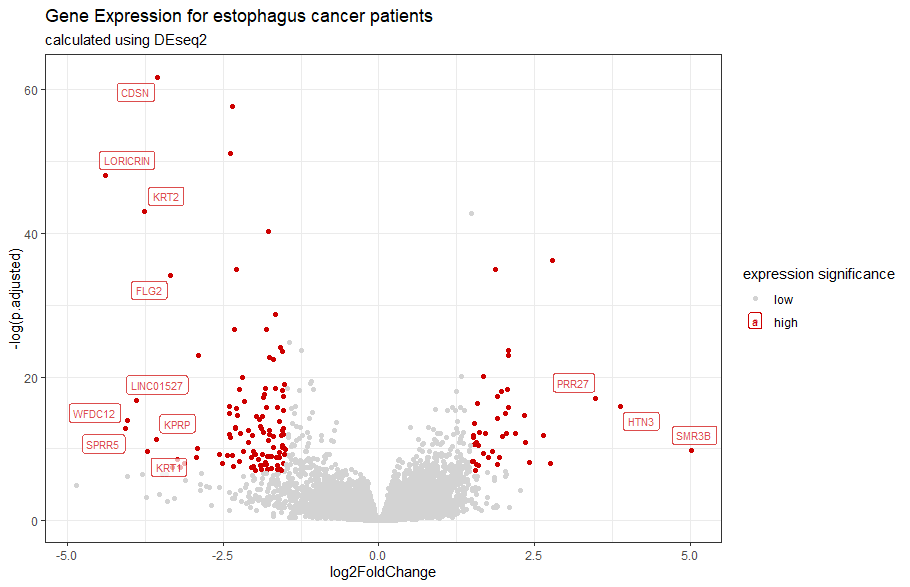
\includegraphics[width=1.2\linewidth]{figures/DEG_result.png}
    \caption{Results of the DEG Analysis}
    \label{fig:DEG-analysis}
\end{figure}

\subsection{Enrichment Analysis}

Enrichment Analysis was applied to the set of 150 genes with significant differential expression (p.adjusted < 0.001 and |Log2FoldChange| > 1.5). The dominant molecular functions (see \ref{fig:ego} a) attributed to the genes with expression changes are \textbf{antigen binding} (overexpressed) and \textbf{peptidase inhibitor activity}. Genes for the latter category show a variety of expression levels; the overexpressed SMR3B (log2FC.=5.0) and the underexpressed  WFDC12 (log2FC.=-4.0) are both in this category. 
The dominant biological function (see \ref{fig:ego} b) attributed to differently expressed genes are \textbf{skin development} and \textbf{keratinocyte differentiation} specifically.  
Relevant Cellular components (see \ref{fig:ego} c) or advanced melanoma are the \textbf{immunoglobulin complex} (place for antigen binding), the \textbf{extracellular matrix} and \textbf{cornified envelope}.


\begin{figure}[h]
    \hspace*{-1in}
    \subfigure[enrichGO: molecular function]{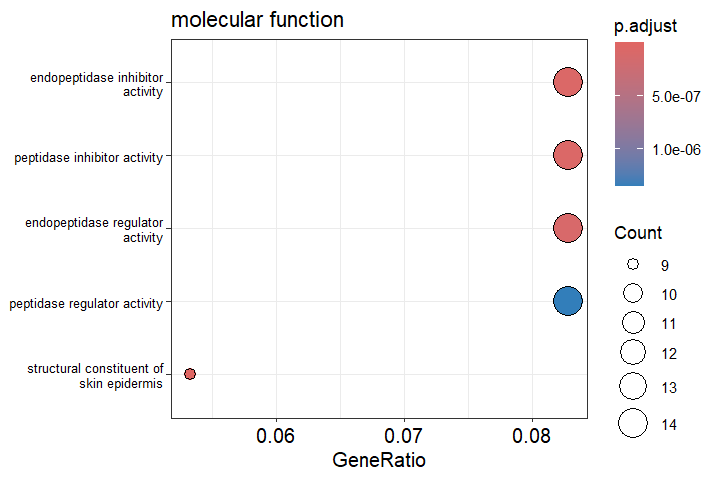
\includegraphics[width=0.6\linewidth]{figures/molecular_function.png}}
    \subfigure[enrichGO: biological function]{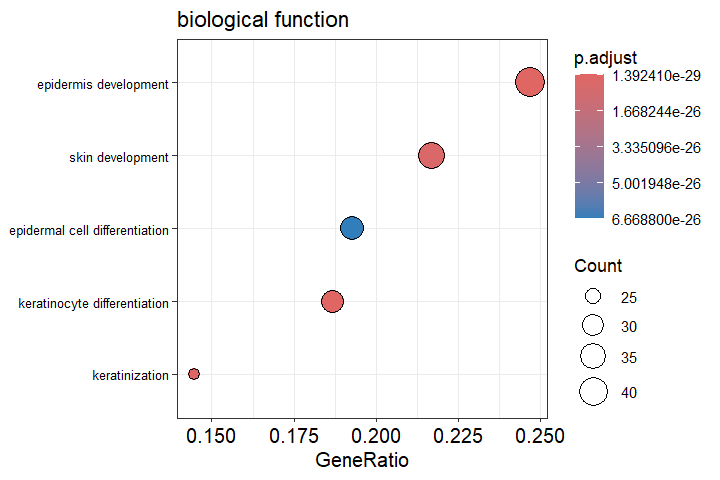
\includegraphics[width=0.6\linewidth]{figures/biological function.png}}
    \hspace*{-1in}
    \subfigure[enrichGO: cellular component]{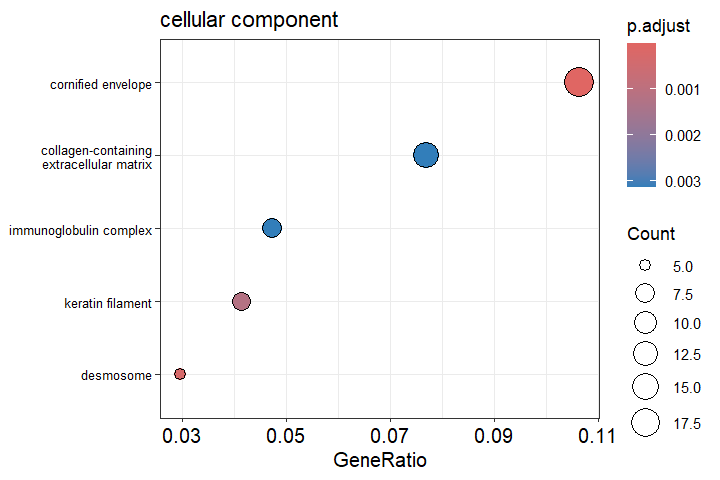
\includegraphics[width=0.6\linewidth]{figures/cellular_component.png}}
    \subfigure[enrichKegg: pathways]{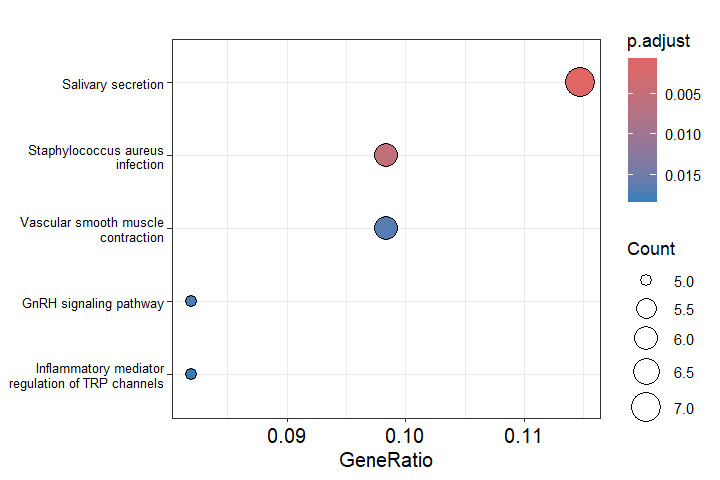
\includegraphics[width=0.6\linewidth]{figures/kegg-pathways.png}}
    \caption{Enrichment Results}
    \label{fig:ego}
\end{figure}


The Kegg pathways (see \ref{fig:ego} c) with highest degree of differential expression are  \textbf{Salivary secretion} interaction (overexpressed), the {Staphylococcus aureus infection} (underexpressed) and \textbf{Vascular smooth muscle contraction} (underexpressed).


\subsection{Discussion}

% We want to study typical criteria of late-stage melenoma on some exemplary genes. 

First, the genes with high degree of differential expression shall be discussed.

LORICRIN is a major component of the cornified envelope of the epidermis \cite{Candi2005}. Keratin-1 (KRT1) and Keratin-2 (KRT2) are both structural proteins that constitute intracellular filaments. \cite{KRT1, KRT2, Candi2005}. Corneodesmosin (CDSN) formes a strong intercellular link to handle mechanical stress in the skin \cite{GARROD2008572}. Filaggrin's (FLG, log2FC=-2.4) purpose is to aggregate and compact Keratin filaments to supplement the cornification of the outer skin layer \cite{ARMENGOTCARBO201586}. Filaggrin-2 (FLG2) is a intercellular link in this cornified skin layer \cite{FLG2}. All these genes encoding proteins that contribute to a strong skin barrier, are underexpressed in late-stage melanoma cells, which are prone to detach and metastate. This requires mobility, which would be hindered by proteins that link to other cells (CDSN and FLG2) or by a stronger intracellular skeleton (Keratin). SPRR5 which positively regulates the differentiation of ceratinozytes \cite{Ziegler2019}, supporting all above mentionend processes,  is also underexpressed. The underexpressed WFDC12  also downregulates formation of Keratin filaments \cite{Kalinina2021}. 

% added alexa: 
Furthermore these proteins are markers for the differentiation of skin cells. Their underexpression could indicate that a dedifferentiaion process takes place. Dedifferentiation of cancer cells into cancer stem cells is a common phenomenon associated with increased drug resistance and metastatic potential \cite{Cancer_dedif_CancerStemCells}. The importance of this process was recently highlighted, as "unlocking phenotypic plasticity", which is enabled via dedifferentiation,  was added to the hallmarks of cancer \cite{hallmarks_new}.

SMR3B inhibits the destruction of proteins, concretely via inhibition of  peptidases and endopeptidases \cite{SMR3B}. Therefore, the overexpressed SMR3B disturbs the protein stress response and can thereby contribute to a malignant metabolism.

Histatins (HTN3) and PRR27 are components of human saliva. Their overexpression in late-stage melanoma has no known relation to cancerous behaviour. Likewise, no effect can be attributed to the underexpression of RNA for the non-coding gene LINC01527.

Only a limited number of highly differentially expressed genes could be discussed specifically, the 150 other significantly differentially expressed genes will be discussed in groups that have been identified in the enrichment analysis.

Genes associated to \textbf{Antigen binding} showed higher expression in late-stage melanoma. Many of these genes are members of the families IGHV and IGKV, which constitute immunglobuline complexes of leukocytes \cite{IGKV}. IGKV genes have been found present in breast cancer cells as well. 

The genes of the DEFB family cytotoxins necessary for fighting a \textbf{Staphylococcus aureus infection}. Their underexpression in late-stage melanoma disables the celular immune reaction to S.aureus, which are known to create a cancer-friendly environment \cite{Staph}. 


%Wu et al. \cite{Wu2021} associate anomalies in the \textbf{calcium signaling} pathway to cancerous  behavior. We have observed accelerated in ribosome genesis for late-stage melanoma. And and increase in cytokine release could be observed, which assumably form an environment suited for cancer proliferation.

% WFDC12 These
% https://www.nature.com/articles/s41419-023-05686-3
% Ich glaube es wäre interessant darauf einzugehen dass WFDC12 runterreguliert ist obwohl Peptidasen an anderer Stelle hochreguliert sind. Mögliche Hypothese auf basis des nature artikel Li et al:
% WFDC12 sorgt in anderen Kontexten (Hautkrankheit AD) für Infiltration von Immunzellen (T Helferzellen). Runter regulation könnte also eventuell der Immunevasion dienen

% Pathview ergenbis einfügen? Zu enrich analyse als Figure:
\begin{figure}[h]
    \centering
    \includegraphics[width=0.9\linewidth]{figures/hsa04970.pathview.png}
    \caption{Differential Expressions in the \textbf{Saliva Secretion} pathway}
    \label{fig:pathviw}
\end{figure}

\section{Summary}

The comparison of gene expression levels between early- and late-stage melanoma yielded interpretable results. Most dominant was the decline in Keratin and other epidermis-constituting proteins which point to the dedifferentiation of the cancerous epidermis cells. Furthermore, the protein stress response was surpressed in late-stage melanoma. Some genes that were intensely underexpressed or overexpressed could could not be attributed any influence on the cancerous behaviour.

%P35 verhindert Zellteilung bei DNA-Schäden


%Loricrin
%https://pmc.ncbi.nlm.nih.gov/articles/PMC10526380/
%We have  previously  shown  that  maintained  expression  of  the  autophagy regulatory protein AMBRA1 (activating molecule in Beclin1-regulated autophagy) and the epidermal differentiation marker loricrin in the epidermis overlying nonulcerated stage I melanomas can identify genuinely low-risk tumour subsets  with  a  negative  predictive  value  of  98.3%.22  The  association  of  tumour  secretion  of  transforming  growth  factor-β2  with  loss  of  peritumoral  AMBRA1  and  reduced  epidermal  integrity  underpins  a  mechanism  of  melanoma  ulceration  and  supports  the  prognostic  value  of  this  bio-marker.23 T
%marker for cell differentiation -> low expression -> cells are in earlier stages of expression




%HTN3: Histatins are found in saliva and exhibit antibacterial, Component of Saliva
%https://www.genecards.org/cgi-bin/carddisp.pl?gene=HTN3
%protein stress response, proliferation activation etc

%PRR27: Proline-rich proteins are major components of parotid and submandibular saliva in humans as well as other animals. [https://pubmed.ncbi.nlm.nih.gov/6810092/]



%überholte Hypothese
%Salivary Gland Cancer might have melanoma metastases. These melanomas could have a high secretion of saliva, because they are derived from Saliva secretion cells. (\cite{Pvalue})
%https://pubmed.ncbi.nlm.nih.gov/1952725/



\newpage
\section{References}

\bibliography{bibliography.bib}


\end{document}